\documentclass{beamer}
\usepackage[utf8]{inputenc}
\usepackage{graphicx}
\usepackage{listings}
\usetheme{Frankfurt}

\lstset{
    language=PHP
   ,basicstyle=\footnotesize
   ,showspaces=false
   ,showstringspaces=false
}

\title{AURA \\ Average User-Response to Attacks}
\author{Mats Börjesson \and Tobias Olausson}
\date{2010-05-21}

\begin{document}

\section{Introduction}

\frame{\titlepage}
\begin{frame}{Aim}
    \begin{itemize}
        \item Implement a small community vulnerable to attacks.
        \item Test these attacks on test subjects.
        \item Record their response to the attacks.
        \item Promote awareness.
    \end{itemize}
\end{frame}

\begin{frame}{Kwitter}
    \begin{columns}[c]
    \begin{column}{.5\textwidth}
        \begin{itemize}
            \item Resembles another large community.
            \item Lets you record status updates.
            \item You are able to see other people's updates aswell.
        \end{itemize}
    \end{column}
    \begin{column}{.5\textwidth}
        
\includegraphics[width=.6\textwidth]{bird.jpg}
    \end{column}
    \end{columns}
\end{frame}

\begin{frame}{Screenshot}
    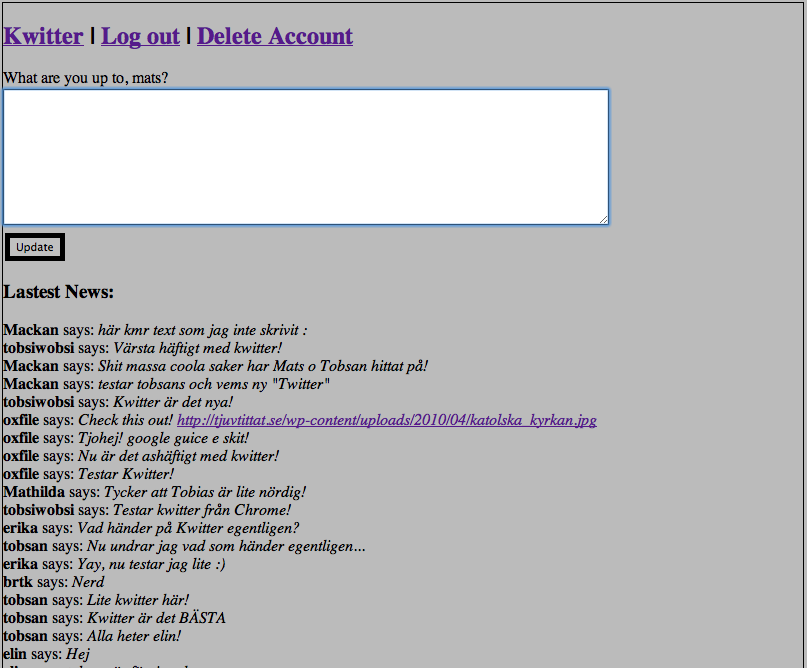
\includegraphics[width=\textwidth]{main.png}
\end{frame}

\section{Implementation}

\begin{frame}{Database}
    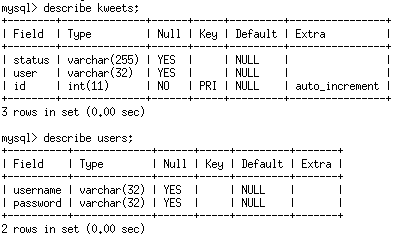
\includegraphics[width=\textwidth]{database.png}
\end{frame}

\begin{frame}[fragile]{Code}
Status update:
\begin{lstlisting} 
if(posted($_POST['status'])) {
    $status = $_POST['status'];
    $user = $_COOKIE['aura'];
    $q = "INSERT INTO kweets VALUES('$status','$user','0')";
    mysql_query($q,$db);
}
\end{lstlisting}
\ldots and status listing
\begin{lstlisting}
$query = "SELECT * FROM kweets ORDER BY id DESC";
$result = mysql_query($query,$db);
if(mysql_num_rows($result) != 0) {
    while($row = mysql_fetch_assoc($result)) {
        $user = $row['user'];
        $status = $row['status'];
        echo "<b>$user</b> says: <i>$status</i><br /> \n";
    }
}
\end{lstlisting}
\end{frame}

\begin{frame}{Attacks}
    \begin{itemize}
        \item Cookie Theft via XSS
        \item Domain Forgery
        \item CSRF (sort of)
        \item SQL-injection (not tested)
    \end{itemize}
\end{frame}

\begin{frame}{Testing}
    \begin{itemize}
        \item User tests
        \item Attacks inserted while testing
        \item Reactions and Response (R'n'R)
    \end{itemize}
\end{frame}

\section{Results}

\begin{frame}{Showtime!}
    \only<1>{Signup \\ 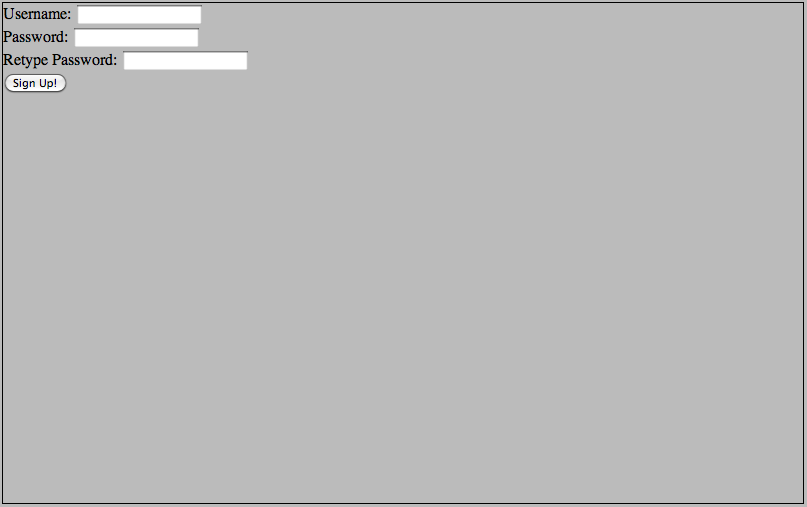
\includegraphics[width=\textwidth]{signup.png}}
    \only<2>{First post \\ 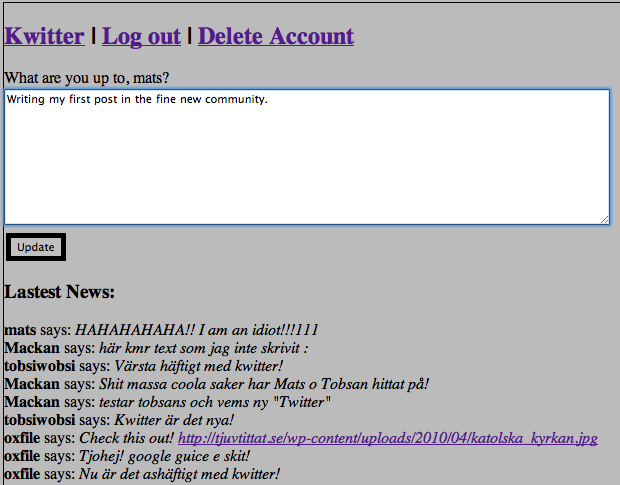
\includegraphics[width=\textwidth]{firstpost.png}}
    \only<3>{Cookie Theft \\ 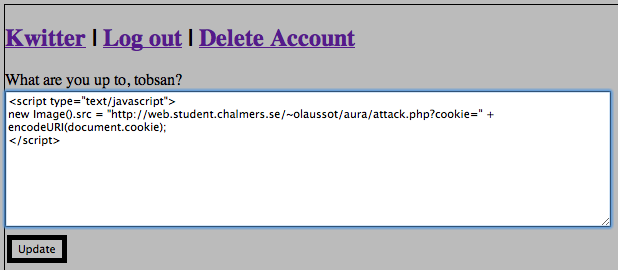
\includegraphics[width=\textwidth]{theft.png}}
    \only<4>{CSRF 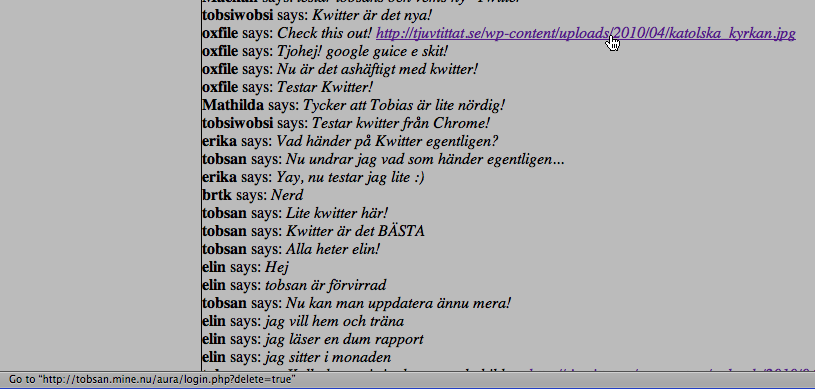
\includegraphics[width=\textwidth]{csrf.png}}
    \only<5>{Redirecting 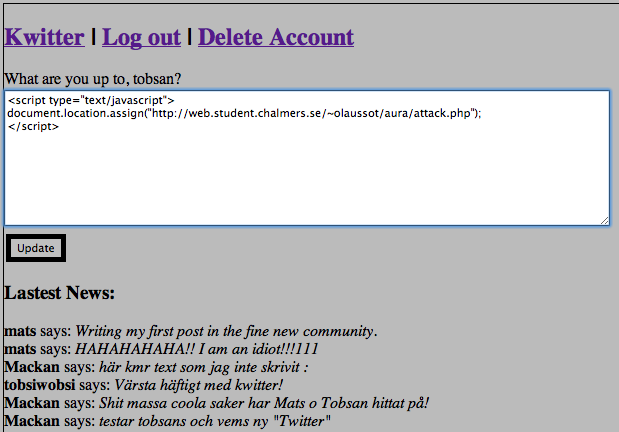
\includegraphics[width=\textwidth]{forgeinject.png}}
    \only<6>{The forged site 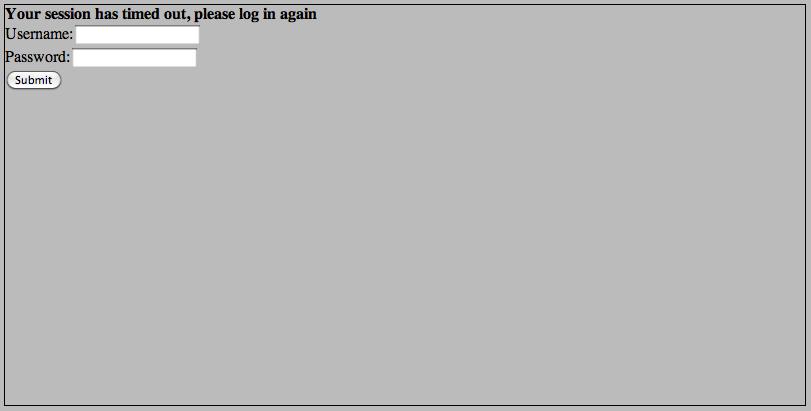
\includegraphics[width=\textwidth]{forgery.png}}
    \only<7>{Possible result after entering info on forged site \\
             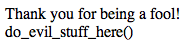
\includegraphics[width=.4\textwidth]{fooled.png}}
\end{frame}

\begin{frame}{Attack success}
    \begin{itemize}
        \item
            The cookie attack is impossible to notice at first. When stolen
            however, it becomes rather obvious that you have been fooled, which
            all subjects noticed.
        \item
            CSRF was way more successful than we thought, almost none of the
            subjects looked where the link actually led before clicking.
        \item
            Domain forgery was not as successful, but this was partly because
            the URL ended in "attack.php".
    \end{itemize}
\end{frame}

\begin{frame}{Response}
    We have tested on 8 persons (mostly CS students)
    \begin{itemize}
        \item None of the subjects realized the domain forgery until it was too
              late.
        \item Around 50\% of the subjects tried clicking the links that led to
              deleting their account without notice.
        \item Most of the subjects however noticed when their cookies were
              stolen.
    \end{itemize}
\end{frame}

\section{Conclusion}

\begin{frame}{Protection}
    \begin{itemize}
        \item Browser protection
        \item Alarm the user!
    \end{itemize}
\end{frame}

\begin{frame}{Be careful!}
    \begin{itemize}
        \item Since most people does not notice these attacks (even though they
              were CS students!), it is more important than ever to protect
              against them.
        \item Also, don't just trust a site because it seems legit, since it may
              still have vulnerabilities. Be suspicious!
    \end{itemize}
\end{frame}

\begin{frame}{Thank you!}
    \begin{columns}[c]
        \begin{column}{.5\textwidth}
            
\includegraphics[height=.8\textheight]{cookies.jpg}
        \end{column}
        \begin{column}{.5\textwidth}
            Contact us: \vspace{1cm}

            \texttt{tobias.olausson@student.gu.se} \\
            \texttt{mats@student.gu.se}
        \end{column}
    \end{columns}
\end{frame}

\end{document}
